\part{Java}
\chapter{Einf�hrung in Java}
%MARK: Kapitel 1 - Siehe java-kap01.pdf im K laufwerk
\section{Hello World in Java}
%PG2(Vorl-Jof)-16.03.2009-DIA1
\begin{figure}[htb]
\begin{tikzpicture}[node distance = 1.5cm, auto]
	\node[draw, rectangle, text centered] (start){Quellprogramm};
	\node[right of=start, node distance = 2.5cm] (startd){Hello.java};
	\node[below of=startd] (startdd){Compilen};

	\node[below of=startdd] (bytecoded){Hello.class};
	\node[left of=bytecoded, draw, rectangle, text centered, node distance = 2.5cm] (bytecode){Bytecode};
	\node[below of=bytecoded] (bytecodedd){java Hello};

	\node[below of=bytecodedd] (ausfuehrend){''Hello''};
	\node[left of=ausfuehrend, draw, rectangle, text centered, node distance = 2.5cm] (ausfuehren){Ausf�hren};

	\draw[->] (start.south) -- (bytecode.north) node[right, midway]{javac};
	\draw[->] (bytecode.south) -- (ausfuehren.north) node[left, midway]{Interpreter} node[right, midway]{java};

	\draw[->] (bytecode.north west) +(-0.5, 0.5) -- (bytecode.north west) node[text width=1.5cm, anchor=south east]{F�r alle CPUs gleich};
\end{tikzpicture}
\end{figure}

\begin{lstlisting}[frame=single, numbers=left, stepnumber=1, numbersep=10pt, language=Java]
//Das erste Programm in der Datei Hello.java
public class Hello {
	public static void main(String[] args) {
		System.out.println("Hello World");
	}
}
\end{lstlisting}
\begin{itemize}
\item Vorsicht:
		\begin{itemize}
		\item Gro�-/Kleinschreibung beachten!
		\item Dateiname = Name der Klasse
				\begin{itemize}
				\item Zusatz zum Dateinamen: java
				\end{itemize}
		\item unbedingt die Schreibweise beachten:
				\begin{itemize}
				\item \lstinline[language=Java]{public static void main(String[] args)}
				\end{itemize}
		\end{itemize}
\item Eclipse ist bei der Programmierung hilfreich
\end{itemize}

\section{Applets}
%PG2(Vorl-Jof)-16.03.2009-DIA1
\begin{figure}[htb]
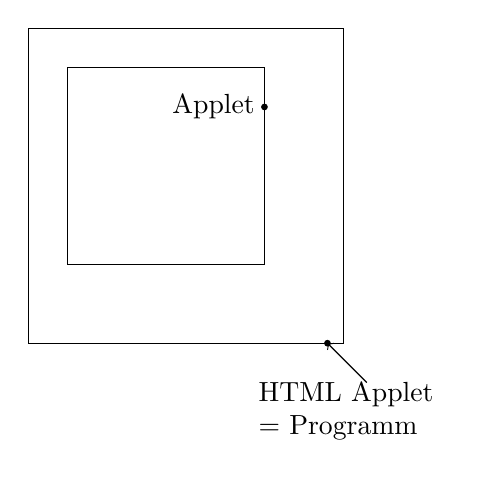
\begin{tikzpicture}
	\draw (0,0) rectangle (4,-4);
	\draw (0.5,-0.5) rectangle (3,-3);

	\draw[fill=black] (3,-1) circle (1pt) node[left] {Applet};
	\draw[fill=black] (3.8,-4) circle(1pt);
	\draw[->] (3.8,-4) +(0.5,-0.5) -- (3.8,-4) node[near start, below, text width=2.5cm] {HTML Applet = Programm};
\end{tikzpicture}
\end{figure}
\begin{itemize}
\item In Java ist der Schritt zu einer Anwendung f�r eine grafische Oberfl�che kein Sprung mehr wie in anderen Systemen.
\item Solche Anwendungen kann man in der Form eines \ac{sog.} \indexi[Applet]{Applets} schreiben.
\item Applets k�nnen analog zu Bildern in .html-Seiten eingebunden werden.
\item Das folgende Applet in Java soll in der Mitte des Bildschirms einen Text ausgeben.
\end{itemize}
\subsection{Hell World f�r Applets (=Mini Anwendung)}
\begin{figure}[htb]
\begin{tikzpicture}
	\draw[-latex] (0,0) -- (6,0) node[below] {$x$};
	\draw[-latex] (0,0) -- (0,-5) node[right] {$y$};

	\draw[fill=lightgray] (0.5,-0.5) rectangle (5.5,-4.5);
	\node[text width=3.5cm] at (3,-2.5) {Mitte \ac{ca.}\\$x$ = \lstinline[language=Java]{getWidth()/2},\\$y$ = \lstinline[language=Java]{getHeight()/2}};
	\node[left, text width=3cm] at (0,0) {Ecke links oben\\$x = 0$, $y = 0$};
	\node[left, above, text width=8cm] at (6,0) {Breite auslesen mit \lstinline[language=Java]{getWidth()}\\H�he auslesen mit \lstinline[language=Java]{getHeight()}\\Dies liefert jeweils die Anzahl Pixel};
	\node[right, text width=3.5cm] at (5.5,-4.5) {Ecke rechts unten\\$x$ = \lstinline[language=Java]{getWidth() - 1}\\$y$ = \lstinline[language=Java]{getHeight() - 1}};
\end{tikzpicture}
\end{figure}

\begin{lstlisting}[frame=single, numbers=left, stepnumber=1, numbersep=10pt, language=Java]
// Ein erstes Applet in Java
import java.applet.Applet;
import java.awt.Graphics;

public class DemoFuerApplet extends Applet {
	public void paint (Graphics g) {
		g.drawString ("Hello World",
		getWidth()/2, getHeight()/2);
	}
}
\end{lstlisting}
Ablauf �ber Eclipse: Run As Java Applet

\section{Zusammenfassung}
\begin{itemize}
\item Java-Programme werden vom Entwickler als Text eingegeben.
\item Die Java-Compiler erzeugen einen Bytecode, der unabh�ngig vom Rechner ist.
\item Java-Programme k�nnen als selbstst�ndige Anwendung laufen, wie man es von anderen Programmiersprachen her gewohnt ist.
\item Java-Programme in Form von sog. Applets k�nnen als Anwendungen von geeigneten Browsern im Rahmen des http-Protokolls vom Server auf Client-Rechner versandt und dort zum Ablauf gebracht werden.
\item Im Rahmen des file-Protokolls ist dies nat�rlich auch auf einem lokalen Rechner m�glich.
\end{itemize}
\begin{itemize}
\item Java ist eine objektorientierte Sprache.
\item Java unterscheidet zwischen Gro�-und Kleinschreibung.
\item Java-Programme beginnen mit einer optionalen Folge von \lstinline[language=Java]{import}-Anweisungen, die die Bez�ge zu anderen Java-Programmen herstellen.
\item Diese \lstinline[language=Java]{import}-Anweisungen sind immer am Anfang des Programms zusammenzustellen.
		\begin{itemize}
		\item \ac{Z.B.} \lstinline[language=Java]{import java.awt.Graphics;}
		\end{itemize}
\item Das Programm wird in Klassen angegeben.
		\begin{itemize}
		\item \ac{Z.B.} \lstinline[language=Java]{class Hello}
		\end{itemize}
\item Diese Klassen k�nnen Methoden enthalten, die den ablauff�higen Teil des Quellprogramms darstellen.
		\begin{itemize}
		\item \ac{Z.B.} main
		\end{itemize}
\end{itemize}

\chapter{Prozedurale Elemente von Java}
%MARK: Kapitel 2 - Siehe java-kap02.pdf im K laufwerk
\section{Grundlagen}
\begin{itemize}
\item Elementare Daten: Variable im Ram
		\begin{itemize}
		\item int: ganze Zahlen
		\item float: Gleitkommazahlen
		\end{itemize}
\item Operatoren: Verarbeitung von Daten
		\begin{itemize}
		\item $+$ $-$ $*$ $/$ $\%$ $>$ $>>$ $>>>$ \ac{etc.}
		\end{itemize}
\item Wertzuweisung als elementare Anweisung
		\begin{itemize}
		\item Zuweisung von Werten an Variable
		\end{itemize}
\item Kontrollfluss: Anweisungen zur Steuerung von Abl�ufen
		\begin{itemize}
		\item \lstinline[language=Java]{if}, \lstinline[language=Java]{switch}: Fallunterscheidungen
		\item \lstinline[language=Java]{do}, \lstinline[language=Java]{while}, \lstinline[language=Java]{for}: Wiederholte Ausf�hrung
		\end{itemize}
\item Methoden: Folgen von Anweisungen
		\begin{itemize}
		\item \lstinline[language=Java]{System.out.println("hello");}
		\end{itemize}
\item Felder: Folgen von Variablen
		\begin{itemize}
		\item \lstinline[language=Java]!int[] zahlen = {30, 5, 2001};!
		\end{itemize}
\end{itemize}

\section{Daten erkl�ren: elementare Datentypen}
\begin{itemize}
\item GanzzahligeDatentypen: ganze Zahlen mit Vorzeichen
\begin{itemize}
		\item \lstinline[language=Java]{byte} 8-Bit-Zahlen von $-128$ bis $+127$ ($-2^7$ bis $2^7-1$)
		\item \lstinline[language=Java]{short} 16-Bit-Zahlen von $-32768$ bis $+32767$ ($-2^{15}$ bis $2^{15}-1$)
		\item \lstinline[language=Java]{int} 32-Bit-Zahlen von $-2147483648$ bis $2147483647$
		\item \lstinline[language=Java]{long} 64-Bit-Zahlen von $-9223372036854775808$ bis $9223372036854775808$
				Beispiel \lstinline[language=Java]{1l}, \lstinline[language=Java]{12345l} (Zusatz \lstinline[language=Java]{l} ist zu beachten, \ac{d.h.} klein-L)
		\end{itemize}
\item Gleitkommazahlen: Nach IEEE-754-Standard
		\begin{itemize}
		\item \lstinline[language=Java]{float} Zahlen mit 32 Bit Genauigkeit. Beispiel: 1.0f (Zusatz f ist zu beachten)
		\item \lstinline[language=Java]{double} Zahlen mit 64 Bit Genauigkeit. Beispiel: 1.0 oder 1.0d
		\end{itemize}
\item Zeichentyp
		\begin{itemize}
		\item \lstinline[language=Java]{char} 16-Bit-Unicode-Zeichen. Beispiel: \lstinline[language=Java]{'A'}, \lstinline[language=Java]{'a'}
		\item Achtung: nur ein einzelnes Zeichen
		\end{itemize}
\item Boolescher Typ
\begin{itemize}
\item \lstinline[language=Java]{boolean} Wahrheitswert. Entweder \lstinline[language=Java]{true} oder \lstinline[language=Java]{false}
\end{itemize}
\item Die elementaren Datentypen werden direkt von der CPU bearbeitet.
\item Die Verarbeitung erfolgt effizient.
\item Dies ist mit ein Grund f�r die relativ gute Performance von Java-Programmen.
\end{itemize}

TODO: Nachtragen von Wolf
